\documentclass[../main.tex]{subfiles}
\begin{document}

%%%%%%%%%%%%%%%%%%%%%%%%%%%%%%%
%%%% sec1
%%%%%%%%%%%%%%%%%%%%%%%%%%%%%%%
\section{Homotop\'ia y caminos}
Para facilitar la siguiente discusi\'on, utilizaremos la notación y nomenclatura de MC.
Veremos que los tipos se comportan como espacios topológicos, y, por lo tanto, también se pueden interpretar como $\infty$-grupoides.
Para esto, recordaremos unas nociones previas.

Dado un espacio topológico $X$, y dos puntos $x,y \in X$, podemos generar el conjunto de caminos de $x$ a $y$.
Sin embargo, este conjunto es muy fino, generalmente no es importante el camino exacto tomado $p$, solo su clase de homotop\'ia $[p]$.

Esto es, la clase de equivalencia bajo la relación $p \htpy q$ si y solo si existe una homotop\'ia entre $p$ y $q$ rel $\partial I$; es decir, que existe una función continua $H:I \times I \to X$ tal que
\[ H(0,t)=x, \quad H(1,t)=y,\quad H(s,0)=p(s),\quad H(s,1)=q(s), \]
donde $I=[0,1]$.

De esta manera, el conjunto relevante es:
\[\text{Hom}_X(x,y)=\{[p] \mid p:I \to X,\; p(0)=x,\; p(1)=y \} \]

Como es conocido, podemos generar una operaci\'on de concatenaci\'on y de camino inverso que respeta las clases de homotop\'ia.
\begin{gather*}
  \ct : \text{Hom}_X(x,y) \times \text{Hom}_X(y,z) \to \text{Hom}_X(x,z)\\
  (\blank)^{-1} : \text{Hom}_X(x,y) \to \text{Hom}_X(y,x)
\end{gather*}
donde la concatenaci\'on es asociativa, tiene como neutro al camino constante $\refl{x}$, y es preservada adecuadamente por funciones continuas.
As\'i, estas operaciones le dan una estructura de grupo a $\text{Hom}_X(x,x)$, el cual es llamado el grupo fundamental de $X$, y es denotado por $\pi_1(X,x)$.

Por otro lado, el espacio $X$ puede ser entendido tambi\'en como una categor\'ia que tiene como objetos los puntos en $X$, y como morfismos caminos de $x,y$ (de ah\'i nuestra notación $\text{Hom}_X(x,y)$).
La concatenaci\'on de caminos es entonces la composición de morfismos, y el camino constante $\refl{x}$ es el morfismo identidad.
Como categor\'ia, $X$ tiene una propiedad adicional, cada morfismo es invertible.

\begin{definition}
  Un \textbf{grupoide} es una categor\'ia en donde todo morfismo es invertible.
\end{definition}

Hemos descrito el grupoide fundamental $\Pi_1(X)$ de $X$, y observamos que el grupo fundamental usual $\pi_1(X,x)$ aparece como la subcategor\'ia completa generada por $\{x\}$.

Pero este solo es el nivel 1 de una jerarquía infinita de homotop\'ias y de estructuras algebraicas.
Una homotop\'ia $H$ usual entre dos caminos $p$ y $q$ puede ser entendida también como una superficie tal que sus bordes coinciden exactamente con $p$ y $q$; es decir, $H$ es un 2-camino entre 1-caminos. Un 3-camino ser\'ia una homotop\'ia entre dos homotop\'ias $H$ y $G$ que mantiene los bordes del 2-camino que generan.

Generalizando, dados dos $n$-caminos $P$ y $Q$ con el mismo borde, definimos por recursi\'on que un ($n+1$)-camino entre $P$ y $Q$, es un mapa $H:I^{n+1}\to X$ tal que $\partial \text{Im}(H)=P \cup Q$.

Se puede verificar que las clases de homotop\'ia de estos $n$-caminos poseen una operación de concatenaci\'on y una operaci\'on que genera caminos inversos, y adem\'as satisfacen algunas reglas adicionales, llamadas \textbf{reglas de coherencia}, las cuales los hacen $n$-grupoides para todo $n \in \Z^+$.
Esto muestra que los espacios topol\'ogicos tienen estructura de $\infty$-grupoides\footnote{Dado que las reglas de coherencia solo se cumplen hasta homotop\'ia, la estructura algebraica generada es de $\infty$-grupoides d\'ebiles; cada vez que hablemos de grupoides nos referiremos a grupoides d\'ebiles.}.

Denotamos la estructura de $n$-grupoide de $X$ por $\Pi_n(X)$.
Y se tiene que, como en el caso del grupo fundamental, $\pi_n(X,x)$ es la subcategor\'ia completa de $\Pi_n(X)$ generada por $x$.

Regresando a DTT, podemos entender una prueba $p$ de que $x=y$ como un camino $p$ de $x$ a $y$.
Las reglas del tipo de identidad nos permiten comparar si dos pruebas (caminos) $p,q:x=_X y$ son iguales entre s\'i; es decir si existe un $r : \id[{(\id[A]{x}{y})}]{p}{q}$. Este es justamente un 2-camino, y de manera an\'aloga podemos iterar infinitamente y observar una estructura de $\infty$-grupoides \cite{curien_weak_2009} \cite{van_den_berg_types_2011}.

En las siguientes secciones, verificaremos expl\'icitamente la estructura de $1$-grupoide de los tipos y caracterizaremos (hasta homotop\'ia) los caminos en algunos de los tipos introducidos en la secci\'on previa.

Veremos que varias definiciones y resultados pueden interpretarse de tres formas distintas, de una forma l\'ogica, de una forma homot\'opica, y de una forma categ\'orica.
Esto se debe a la correspondencia Curry-Howard, al hecho de que los tipos corresponden a tipos de homotop\'ia de espacios topológicos y al hecho de que también son $\infty$-grupoides, respectivamente.


%%%%%%%%%%%%%%%%%%%%%%%%%%%%%%%
%%%% sec2
%%%%%%%%%%%%%%%%%%%%%%%%%%%%%%%
\section{Los tipos son 1-grupoides}
Desagregamos todas las condiciones que se deben cumplir para que los tipos sean 1-grupoides como descrito en la secci\'on previa:

\begin{enumerate}
  \item Existe la composición de morfismos $\ct$.
  \item Para cada objeto $x$, existe un morfismo identidad $c_x$ tal que $c_x \ct f = f \ct c_y = f$ para todo $f:x \to y$.
  \item La composición de morfismos es asociativa.
  \item Existe un morfismo $f^{-1}$ inverso para cada morfismo $f:x \to y$, tal que $f^{-1} \ct f=c_y$ y $f \ct f^{-1}=c_x$.
\end{enumerate}

Las primeras tres condiciones vienen de los axiomas de una categor\'ia, mientras que el \'ultimo es la condici\'on de un grupoide. Procederemos a demostrar estas condiciones en orden.

\begin{lemma}
  Para todo tipo $A$ y todo $x,y,z:A$ existe la función de concatenaci\'on de caminos
  \begin{equation*}
    {\blank} \ct {\blank} : (x= y) \to (y= z) \to (x=  z),
  \end{equation*}
  tal que $\refl{x}\ct \refl{x}\jdeq \refl{x}$.
\end{lemma}

N\'otese que visto l\'ogicamente, este lema enuncia la propiedad de transitividad de la igualdad.
Probaremos este lema dos veces; la primera, usando el principio de inducci\'on del tipo de identidades, y la segunda, usando b\'usqueda de patrones, a fin de comparar estos dos m\'etodos.

\begin{proof}[Demostración por inducción]
  Definiremos una funci\'on $f : \prd{x,y:A} (x= y) \to \prd{z:A} (y= z)\to (x=  z)$ por inducci\'on. Sea $D:\prd{x,y:A} (x=y) \to \type$ la familia de tipos definida por
  \begin{equation*}
    D(x,y,p)\defeq \prd{z:A}{q:y=z} (x=z).
  \end{equation*}
  N\'otese que $D(x,x,\refl x) \jdeq \prd{z:A}{q:x=z} (x=z)$.
  Para obtener un elemento de este tipo, volveremos a aplicar inducción, sea $E:\prd{x,z:A}{q:x=z}\to \UU$ la familia de tipos definida por $E(x,z,q)\defeq (x=z)$.
  Podemos definir
  \begin{equation*}
    e(x) \defeq \refl{x} : E(x,x,\refl{x})
  \end{equation*}
  Por lo tanto, obtenemos una funci\'on
  \begin{gather*}
    d : \prd{x,z:A}{q:x=z} E(x,z,q) \\
    d \defeq \ind{=_A}(E, e)
  \end{gather*}
  Con esta funci\'on, podemos definir
  \begin{gather*}
    f : \prd{x,y:A}{p:x=y} D(x,y,p) \\
    f \defeq \ind{=_A}(D, d)
  \end{gather*}
  Finalmente, podemos definir
  \[ p \ct q \defeq f(x,y,p,z,q) \]
  Adem\'as, se tiene que
  \begin{align*}
    \refl{x} \ct \refl{x} & \jdeq f(x,x,\refl{x},x,\refl{x} )            \\
                          & \jdeq \ind{=_A}(D,d,x,x,\refl{x},x,\refl{x}) \\
                          & \jdeq d(x,x,\refl{x})                        \\
                          & \jdeq \ind{=_A}(E,e,x,x,\refl{x})            \\
                          & \jdeq e(x)                                   \\
                          & \jdeq \refl{x}
  \end{align*}
\end{proof}

\begin{proof}[Demostración por b\'usqueda de patrones]
  Buscamos una función
  \[{\blank} \ct {\blank} : (x= y) \to   (y= z)\to (x=  z)\]
  Podemos asumir que $y$ es $x$ y que el primer camino es $\refl{x}$, por lo que reducimos la tarea a encontrar una función ${\refl{x}} \ct {\blank} : (x= z) \to (x=  z)$.

  Nuevamente, podemos asumir que $z$ es $x$ y el segundo camino tambi\'en es $\refl{x}$, con lo que solo es necesario encontrar un elemento de $(x=x)$. Tomando $\refl{x}:x=x$, podemos definir $\ct$ por $\refl{x} \ct \refl{x}\defeq \refl{x}$.
\end{proof}

Es claro que la segunda prueba, aunque omite ciertos detalles, es mucho m\'as legible que la primera, mientras que conserva suficiente informaci\'on para ser entendible.
En efecto, los asistentes de prueba pueden inferir correctamente todos los datos omitidos.
Por estos motivos, este es el estilo que tomaremos en las siguientes demostraciones.

\begin{lemma}\label{reflright}
  Para todo tipo $A$, $x,y:A$ y $p:x=y$, se tiene que $\refl{x} \ct p = p$ y $p \ct \refl{y} = p$.
\end{lemma}
\begin{proof}
  Podemos asumir que $p$ es $\refl{x}$, por lo que ambas ecuaciones se reducen a $\refl{x} \ct \refl{x} = \refl{x}$, lo cual se da por definición de $\ct$.
\end{proof}

Este lema muestra que $\refl{x}$ toma el rol del camino constante, y genera dos 2-caminos $\mathsf{refl\text{-}left}: \id[{(\id[A]{x}{y})}]{\refl{x} \ct p}{p}$ y $\mathsf{refl\text{-}right}: \id[{(\id[A]{x}{y})}]{p \ct \refl{y}}{p}$.
No nombraremos a todos los $n$-caminos que definiremos expl\'icitamente.

\begin{lemma}\label{assoc}
  Para todo tipo $A$, $x,y,z,w:A$, $p:x=y$, $q:y=z$ y $r:z=w$ se tiene $(p \ct q) \ct r = p \ct (q \ct r)$.
\end{lemma}
\begin{proof}
  A trav\'es de repetidas aplicaciones de b\'usqueda de patrones, podemos asumir que $p,q$ y $r$ son $\refl{x}$, por lo que la ecuaci\'on se reduce a $(\refl{x} \ct \refl{x}) \ct \refl{x} = \refl{x} \ct (\refl{x} \ct \refl{x})$, lo cual se da por definición de $\ct$.
\end{proof}

Dado este \'ultimo lema, no utilizaremos paréntesis cuando haya una concatenaci\'on de varios caminos, como es com\'un en \'algebra.

\begin{lemma} \label{-1lema}
  Para todo tipo $A$, $x,y:A$, y $p:x=y$, existe un $p^{-1}:y=x$, y este satisface que $p^{-1} \ct p=\refl{y}$ y $p \ct p^{-1}=\refl{x}$.
\end{lemma}
\begin{proof}
  Asumiendo que $p$ es $\refl{x}$, ponemos $\refl{x}^{-1}\defeq \refl{x}$.
  En este caso, las dos ecuaciones se reducen a $\refl{x} \ct \refl{x} = \refl{x}$, lo cual se da por definición de $\ct$.
\end{proof}

N\'otese que el camino inverso representa el hecho l\'ogico de que las igualdades son sim\'etricas.
Juntando estos lemas, obtenemos:

\begin{theorem}
  Los tipos son 1-grupoides, siendo los elementos los objetos, y los caminos $p:x=y$ los morfismos.
\end{theorem}

Otros dos resultados clásicos y útiles, que se derivan de las reglas de 1-grupoides, son:
\begin{lemma}
  Para todo tipo $A$, $x,y,z:A$, y $p:x=y$, $q:y=z$, se tiene que $(p^{-1})^{-1}=p$ y $(p \ct q )^{-1} = q^{-1} \ct p^{-1}$.
\end{lemma}
\begin{proof}
  Asumiendo que $p$ y $q$ son $\refl{x}$, ambos lados de ambas expresiones se reducen a $\refl{x}$.
\end{proof}

Resaltamos que, a diferencia de en topolog\'ia, la operación de concatenaci\'on y de inversas ha sido definida uniformemente para todos los caminos.
As\'i, inmediatamente todos que los resultados previos, y los de las pr\'oximas secciones, aplican para cualquier $n$-camino.

%%%%%%%%%%%%%%%%%%%%%%%%%%%%%%%
%%%% sec3
%%%%%%%%%%%%%%%%%%%%%%%%%%%%%%%
\section{Funciones y functores}
En topolog\'ia algebraica, es sabido que las funciones continuas entre espacios topológicos inducen un homomorfismo de grupos entre los grupos fundamentales.
Pero m\'as es cierto, las funciones continuas inducen un homomorfismo de $\infty$-grupoides.

Este es el caso tambi\'en para las funciones no dependientes en DTT; verificaremos este hecho para la estructura de $1$-grupoides.
Comenzamos con las funciones no dependientes.

\begin{lemma}\label{aplema}
  Sea $f:A \to B$ una funci\'on, para todo $x,y:A$ existe una función
  \begin{equation*}
    \apfunc f : (\id[A] x y) \to (\id[B] {f(x)} {f(y)}).
  \end{equation*}
  tal que para todo $x:A$, se tiene que $\apfunc{f}(\refl{x})\jdeq \refl{f(x)}$.
\end{lemma}
\begin{proof}
  Asumiendo que el camino del dominio es $\refl{x}$, necesitamos encontrar un camino $f(x)=_B f(x)$, pero tenemos que $\refl{f(x)}$ es un elemento de este tipo.
\end{proof}

\begin{notation}\label{ap}
  En algunos casos, escribiremos $f(p)$ o $fp$ en vez de $\apfunc f (p)$, como es com\'un en teor\'ia de categor\'ias.
\end{notation}

L\'ogicamente, $\apfunc f$ refleja el hecho obvio de que la igualdad es preservada bajo aplicaci\'on de funciones.
Topol\'ogicamente, vemos que las funciones llevan caminos a caminos, lo que nos indica cierta noci\'on de continuidad de todas las funciones. En efecto, las funciones entre tipos corresponden a funciones continuas entre tipos de homotop\'ias de espacios topol\'ogicos.
Categ\'oricamente, como sugerido por la Notaci\'on \ref{ap}, las funciones corresponden a functores entre grupoides.

\begin{lemma}\label{apct}
  Sea $f:A \to B$ una funci\'on, y $p:\id[A]{x}{y}$ y $q:\id[A]{y}{z}$ dos caminos en $A$, entonces
  \begin{equation*}
    \apfunc f (p \ct q) = \apfunc{f}(p) \ct \apfunc{f}(q)
  \end{equation*}
\end{lemma}
\begin{proof}
  Asumiendo que $p$ y $q$ son $\refl{x}$, ambos lados se reducen a $\refl{f(x)}$, por definición de $\ct$ y $\apfunc{f}$.
\end{proof}

Con el Lema \ref{aplema} en mano, podemos aplicar un razonamiento algebraico sobre los caminos:

\begin{lemma}
  Sea $f:A \to B$ una funci\'on, y $p:\id[A]{x}{y}$ un camino, entonces se tiene que $(f(p))^{-1}=f(p^{-1})$
\end{lemma}
\begin{proof}
  El Lema \ref{-1lema} nos da un camino $q_1:p^{-1} \ct p = \refl{y}$. Entonces, definiendo
  \begin{gather*}
    g:(y=y) \to (f(y)=f(y)) \\
    g(r)\defeq \apfunc f (r),
  \end{gather*}
  obtenemos un camino $$g(q_1): f(p^{-1} \ct p) = \refl{f(y)}$$
  Por otro lado, el Lema \ref{apct} nos da un camino $q_2: f(p^{-1} \ct p) = f(p^{-1}) \ct f(p)$.

  Juntando estos resultados, obtenemos que
  $$q_2^{-1} \ct g(q_1) : f(p^{-1}) \ct f(p) = \refl{f(y)}$$
  Definiendo
  \begin{gather*}
    h_1:(f(y)=f(y))\to (f(y)=f(x)) \\
    h_1(r)\defeq r \ct (f(p))^{-1},
  \end{gather*}
  obtenemos
  $$h_1(q_2^{-1} \ct g(q_1)) : \left(f(p^{-1}) \ct f(p)\right) \ct (f(p))^{-1}= \refl{f(y)}\ct \left(f(p)\right)^{-1}$$
  Por el Lema \ref{reflright}, tenemos caminos
  \begin{gather*}
    q_3: f(p^{-1}) \ct \refl{f(x)} = f(p^{-1})\\
    q_4:\refl{f(y)}\ct \left(f(p)\right)^{-1} = \left(f(p)\right)^{-1}
  \end{gather*}
  Por el Lema \ref{-1lema}, tenemos el camino
  \[ q_5:f(p) \ct (f(p))^{-1} = \refl{f(x)}\]
  Poniendo
  \begin{gather*}
    h_2:(f(x)=f(x))\to (f(y)=f(x)) \\
    h_2(r)\defeq f(p^{-1}) \ct r,
  \end{gather*}
  vemos que
  \[ h_2(q_5) : f(p^{-1}) \ct\left( f(p) \ct (f(p))^{-1} \right)= f(p^{-1}) \ct\refl{f(x)}\]
  Por el Lema \ref{assoc}, existe un camino
  \[q_6:\left(f(p^{-1}) \ct f(p)\right) \ct (f(p))^{-1}= f(p^{-1}) \ct \left( f(p) \ct (f(p))^{-1}\right)\]
  Juntando estos resultados previos, obtenemos:
  \begin{align*}
    \left(f(p)\right)^{-1}                  &
    = \refl{f(y)}\ct \left(f(p)\right)^{-1} &                                                    & \text{Por $q_4^{-1}$}                                                \\
                                            & = \left(f(p^{-1}) \ct f(p)\right) \ct (f(p))^{-1}  &                       & \text{Por $(h_1(q_2^{-1} \ct g(q_1)))^{-1}$} \\
                                            & = f(p^{-1}) \ct \left( f(p) \ct (f(p))^{-1}\right) &                       & \text{Por $q_6$}                             \\
                                            & = f(p^{-1}) \ct\refl{f(x)}                         &                       & \text{Por $h_2(q_5)$}                        \\
                                            & = f(p^{-1})                                        &                       & \text{Por $q_3$}
  \end{align*}
  Nótese que esta cadena de igualdades corresponde en realidad a la siguiente concatenación de caminos:
  \[ (q_4)^{-1} \ct (h_1(q_2^{-1} \ct g(q_1)))^{-1} \ct q_6 \ct h_2(q_5) \ct q_3 : (f(p))^{-1}=f(p^{-1}) \]
\end{proof}

Utilizaremos la práctica común de escribir la cadena de igualdades, dejando implícito el camino específico que se est\'a usando, solo haciendo referencia al resultado previo del cual este se deriva, si es necesario.

Hemos construido un 2-camino espec\'ifico en la demostración del lema anterior, pero n\'otese que este no es \'unico.
Pudimos, por ejemplo, utilizar inducción sobre $p$.
Uno esperar\'ia que estos dos 2-caminos sean iguales; es decir, que existe un 3-camino que los relaciona.
Este es efectivamente el caso, como se puede ver por inducción, y es una de las consecuencias de las reglas de coherencia de un $2$-grupoide.

No obstante, trabajar con las reglas de coherencia de $n$-caminos para $n \geq 2$ se vuelve r\'apidamente muy complicado.
Veremos luego que en varios casos es posible reducir una pregunta sobre $n$-caminos, a una de $1$-caminos, por lo que nuestro \'enfasis es en estos.

Otros resultados útiles e inmediatos son los siguientes:

\begin{lemma}
  Sean $f:A \to B$ y $g:B \to C$ funciones, y $p:\id[A]{x}{y}$ un camino, entonces se tiene:
  \begin{enumerate}
    \item $\apfunc{(g \circ f)}(p) = (\apfunc g \circ \apfunc f)(p)$
    \item $\apfunc \idfunc (p) = p$
    \item Sean $q,r: \id[A]{y}{z}$, con $p \ct q = p \ct r$, entonces $q = r$
    \item Sean $q: \id[A]{x}{y}$ y $r:\id[A]{y}{z}$, con $p \ct r = q \ct r$, entonces $p = q$
  \end{enumerate}
\end{lemma}
\begin{proof}
  Para $(I)$ y $(II)$, asumiendo que $p$ es $\refl{x}$, ambos lados se reducen a $\refl{x}$.
  Para $(III)$ y $(IV)$, estos son consecuencia del Lema \ref{reflright}, cuando asumimos que $p$ y $r$ son $\refl{y}$, respectivamente.
\end{proof}

%%%%%%%%%%%%%%%%%%%%%%%%%%%%%%%
%%%% sec4
%%%%%%%%%%%%%%%%%%%%%%%%%%%%%%%
\section{Funciones dependientes y fibraciones}
Sea $f:\dprd{x:A}B(x)$ una función dependiente, dado un camino $p:x=y$, se podr\'ia esperar que se tenga también un camino en $f(x)=f(y)$.
Sin embargo, inspecci\'on de este \'ultimo t\'ermino muestra que este no tiene sentido: $f(x)$ est\'a en $B(x)$, mientras que $f(y)$ est\'a en $B(y)$, y caminos entre tipos diferentes no est\'a definido.
Lo que necesitamos es una forma de relacionar estos dos tipos, la función transporte nos brinda esta posibilidad.

\begin{lemma}[Transporte]
  Sea $B$ una familia de tipos sobre $A$, y sea $p:\id[A]{x}{y}$ un camino, entonces existe una función
  $$\trfib{B}{p}{\blank} : B(x) \to B(y) $$
\end{lemma}
\begin{proof}
  Podemos asumir que $p$ es $\refl{x}$, en cuyo caso necesitamos una función $B(x) \to B(x)$, tomamos a la función identidad $\idfunc[B(x)]$ para esto.
\end{proof}

Entendiendo $B$ como una propiedad que un elemento puede tener, el lema previo nos dice que, si $x$ y $y$ son iguales, entonces $B(x)$ implica $B(y)$. Aplicando el transporte en el camino inverso, obtenemos que $B(x)$ y $B(y)$ son l\'ogicamente equivalentes. As\'i, podemos ``transportar'' propiedades $B$ que tenga un elemento $x$ a un elemento $y$ que sea igual a este.

Categ\'oricamente, vemos que tenemos otra categor\'ia cuyos objetos son de la forma $B(x)$ para alg\'un $x:A$, y los morfismos son funciones $f: B(x) \to B(y)$.
La función transporte entonces lleva morfismos de $A$ (visto como una categor\'ia) a morfismos en esta nueva categor\'ia presentada.
Como uno esperar\'ia, el transporte es un functor (contravariante):

\begin{lemma} \label{trfunctor}
  Sea $B$ una familia de tipos sobre $A$, y sean $p:\id[A]{x}{y}$ y $q:\id[A]{y}{z}$ caminos, entonces
  \[\trfib{B}{p \ct q}{\blank} = \trfib{B}{q}{\blank} \circ \trfib{B}{p}{\blank} \]
\end{lemma}
\begin{proof}
  Podemos asumir que $p$ y $q$ son $\refl{x}$, en cuyo caso la ecuaci\'on se reduce a $\idfunc[B]=\idfunc[B] \circ \idfunc[B]$, y podemos tomar $\refl{\idfunc[B]}$.
\end{proof}

Aunque el punto de vista categ\'orico nos brinda mucha informaci\'on, es a\'un m\'as \'util considere la perspectiva homot\'opica la cual presentamos a continuaci\'on.

Dada una familia de tipos $B:A \to \UU$, la idea es considerar el tipo $B(x)$ como la fibra sobre $x$, como se ve en la Figura \ref{fig-fibras}.
En efecto, en la primera proyecci\'on $\fst: \tsm{x:A}B(x) \to A$, aquellos elementos que son mapeados a $a$ son justamente de la forma $(a,y)$, por lo que podemos identificarlos con los elementos $y:B(a)$. Es m\'as, se puede demostrar que este concepto de fibra es equivalente al concepto usual de preimagen (ver Proposici\'on \ref{fibras-eq}).

\begin{figure}[h]
  \caption{Tipos de familias como fibras}
  \centering
  \vspace{1em}
  \includegraphics[width=0.5\textwidth]{images/fibras}
  \label{fig-fibras}
\end{figure}

Con esta imagen en mente, dado un camino $p:x=y$, vemos que la función transporte induce una función entre las fibras $B(a)$ y $B(y)$, tal que la concatenaci\'on de caminos respeta la composición de las funciones inducidas.
As\'i, un camino puede ser ``levantado'' a una funci\'on entre fibras.

Otra noci\'on a\'un m\'as importante de levantamiento, es la de levantamiento de caminos.
Como ya mencionamos, no puede haber un camino entre elementos de $u:B(x)$ y $v:B(y)$ pues son tipos distintos, pero s\'i puede haber un camino entre los elementos $(x,u),(y,v):\tsm{x:A}B(x)$.

\begin{definition}
  Sea $B:A\to \UU$ una familia de tipos. Diremos que un camino $q:\id[\sm{x:A}B(x)]{(x,u)}{(y,v)}$ est\'a sobre $p:x=y$, si $\fst(q) = p$. Utilizaremos la notaci\'on $q: u =_p^B v$ para estos casos.
\end{definition}

Con esta definici\'on, podemos enunciar la siguiente propiedad.

\begin{lemma}(Propiedad de levantamiento de caminos)\label{path-lift}
  Sea $B:A\to \UU$ una familia de tipos y sea $u:B(x)$ para alg\'un $x:A$. Entonces, para todo $p:x=y$ tenemos un camino
  \[ \mathsf{lift}(u,p): (x,u) = (y, \trfib{B}{p}{u}) \]
  tal que $\mathsf{lift}(u,p)$ est\'a sobre $p$.
\end{lemma}
\begin{proof}
  Podemos asumir que $p$ es $\refl{x}$, en cuyo caso necesitamos una igualdad $(x,u)=(y,{\trfib{B}{\refl{x}}{u}})$, pero el lado derecho de esta igualdad es $(x,u)$, por lo que podemos tomar $\refl{(x,u)}$.

  Para ver que $\fst(\mathsf{lift}(u,p))=p$, supongamos nuevamente que $p$ es $\refl{x}$, entonces nos queda probar $\apfunc \fst \left(\refl{(x,u)}\right)=\refl{x}$. Pero esto es cierto por definición de $\mathsf{ap}$.
\end{proof}

Aunque esta noci\'on de caminos es muy natural y permite expresar y probar varias propiedades, no es muy f\'acil de manejar.
Notando que existe un camino can\'onico $\mathsf{lift}(u,p):(x,u) = (y, \trfib{B}{p}{u})$, entonces vemos que todo camino $q:(x,u)=(y,v)$ sobre $p:x=y$ factoriza por $\mathsf{lift}(x,u)$ a un camino $r:(y , \trfib{B}{p}{u})=(y,v)$ sobre el camino constante en $y$, ver Figura \ref{caminos-sobre}.
An\'alogamente, todo camino $r:(y , \trfib{B}{p}{u})=(y,v)$ sobre $\refl{y}$ puede ser expandido a un camino $q:(x,u)=(y,v)$ sobre $p$, pre-concatenando con $\mathsf{lift}(x,u)$.

\begin{figure}[h]
  \caption{Caminos sobre caminos}
  \centering
  \vspace{1em}
  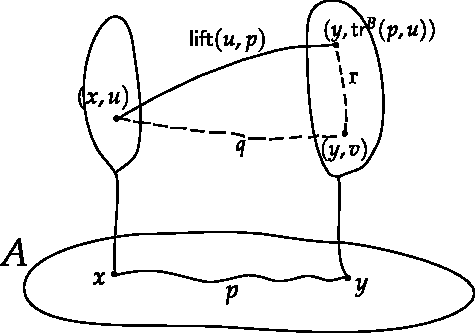
\includegraphics[width=0.6\textwidth]{images/caminoslevantados}
  \label{caminos-sobre}
\end{figure}

Mostraremos luego que esta correspondencia es en realidad una equivalencia (Proposici\'on \ref{paths-over-def}); es decir, tenemos que
\[ \eqv{\left(\id[\sm{x:A}B(x)]{(x,u)}{(y,v)}\right)}{\left(\id[B(y)]{\trfib{B}{p}{u}}{v}\right)} \]

El tipo de la derecha es mucho m\'as manejable por lo que ser\'a el que utilizaremos para las aplicaciones.

Recordemos que una \textbf{fibraci\'on} $p:E \to X$ es un mapa que puede levantar cualquier homotop\'ia en $X$ hacia una en $E$.
Con el lema previo, vemos entonces la relevancia del tipo $\tsm{x:A}B(x)$ en la perspectiva homot\'opica.
El hecho de que haya una proyecci\'on $\fst: \tsm{x:A}B(x) \to A$, y que adem\'as tenemos esta propiedad de levantamiento de caminos, nos da indicios de que $\fst$ es una fibraci\'on, con espacio total $\tsm{x:A}B(x)$.
Este es efectivamente el caso, y es demostrado en la Proposici\'on \ref{sigmafib}.

Dado esto, podemos entender a las funciones dependientes $f:\tprd{x:A}B(x)$ como \textbf{secciones}, pues toman un elemento de cada fibra $B(x)$. Como se esperar\'ia, dada una secci\'on $f:\tprd{x:A}B(x)$, es posible levantar caminos $p:x=y$ a caminos $p':f(x)=_p^B f(y)$.

\begin{lemma} \label{apd}
  Sea $f: \dprd{x:A}B(x)$ una funci\'on dependiente, entonces existe una función
  $$\apdfunc f : \dprd{p:x=y} \left(\id[B(y)]{\trfib{B}{p}{f(x)}}{f(y)}  \right) $$
\end{lemma}
\begin{proof}
  Podemos asumir que $p$ es $\refl{x}$, en cuyo caso necesitamos una igualdad $\id[B(x)]{\trfib{B}{\refl{x}}{f(x)}}{f(x)}$, pero el lado izquierdo de esta igualdad es $f(x)$, por lo que podemos tomar $\refl{f(x)}$.
\end{proof}

Finalmente, retomando la perspectiva categ\'orica, vemos que el transporte tiene una propiedad asociatividad con las funciones (vistas como functores):

\begin{lemma}\label{tr-funcs}
  Sea $B : A \to \UU$ una familia de tipos sobre el tipo $A$, y sea $f:A \to A$ una funci\'on. Para todos $x,y :A$ y $p:x=y$ se tiene
  \[ \trfib{B}{f(p)}{\blank} = \trfib{B \circ f}{p}{\blank}\]
\end{lemma}
\begin{lemma}\label{tr-funcs-id}
  Sea $B : A \to \UU$ una familia de tipos sobre el tipo $A$. Para todos $x,y :A$ y $p:x=y$ se tiene
  \[ \trfib{\idfunc}{B(p)}{\blank} = \trfib{B}{p}{\blank}\]
\end{lemma}
\begin{proof}
  Por inducción en $p$, ambos lados de ambas ecuaciones se reducen a la funci\'on identidad.
\end{proof}

%%%%%%%%%%%%%%%%%%%%%%%%%%%%%%%
%%%% sec5
%%%%%%%%%%%%%%%%%%%%%%%%%%%%%%%
\section{Equivalencias homot\'opicas}\label{sec-equivs}
En MC, dos funciones son homot\'opicas cuando existe una deformaci\'on continua de sus im\'agenes.
Dicho de otra forma, existe una función continua que une uniformemente las dos im\'agenes de cada punto en el dominio a trav\'es de un camino.
Podemos generalizar esto para funciones dependientes:

\begin{definition}
  Sean $f,g:\tprd{x:A}P(x)$ dos secciones. Una \textbf{homotop\'ia} entre estas es una funcio\'n $H$ en el tipo
  \[(f\htpy g) \defeq \prd{x:A}(f(x)=g(x))\]
  Diremos que $f$ y $g$ son homot\'opicas cuando tengamos $f\htpy g$.
\end{definition}

Es claro que la propiedad de ser homot\'opicas es una relaci\'on de equivalencia, pues esto sigue del hecho de que las igualdades son una relaci\'on de equivalencia.

Desde la perspectiva l\'ogica, una homotop\'ia dice que dos funciones son iguales en cada punto del dominio.
Categ\'oricamente, una homotopía es una transformación natural.


\begin{lemma}\label{htpy-nattrans}
  Sea $H:f\htpy g$ una homotop\'ia entre las funciones $f,g:A\to B$, y sea $p:\id[A]xy$.
  Entonces tenemos
  \begin{equation*}
    H(x)\ct\ap{g}{p}=\ap{f}{p}\ct H(y).
  \end{equation*}
  Diagram\'aticamente,
  \[\begin{tikzcd}
      {f(x)} & {f(y)} \\
      {g(x)} & {g(y)}
      \arrow["{H(y)}", from=1-2, to=2-2]
      \arrow["{g(p)}"', from=2-1, to=2-2]
      \arrow["{H(x)}"', from=1-1, to=2-1]
      \arrow["{f(p)}", from=1-1, to=1-2]
    \end{tikzcd}\]
\end{lemma}
\begin{proof}
  Por inducci\'on, podemos suponer que $p$ es $\refl x$.
  Entonces, es suficiente demostrar
  \[ H(x) \ct \refl{g(x)} = \refl{f(x)} \ct H(x). \]
  Pero tenemos que ambos lados son iguales a $H(x)$.
\end{proof}

En topolog\'ia cl\'asica, cuando para una funci\'on $f:A \to B$ existe otra funci\'on $g:B\to A$ tal que $f\circ g \htpy \idfunc[B]$ y $g\circ f \htpy \idfunc[A]$, decimos que $A$ y $B$ tienen el mismo tipo de homotop\'ia, y $f$ es llamada una equivalencia homot\'opica.
En DTT, esto corresponder\'ia a afirmar que el siguiente tipo est\'a habitado.
\begin{equation*}
  \mathsf{qinv}(f) \defeq \sm{g:B\to A} \big((f \circ g \htpy \idfunc[B]) \times (g\circ f \htpy \idfunc[A])\big)\label{eq:qinvtype}
\end{equation*}

Categ\'oricamente, y recordando que las homotop\'ias son transformaciones naturales, este tipo indica la existencia de una equivalencia de categor\'ias entre $A$ y $B$.
Sin embargo, este tipo no corresponde adecuadamente al concepto equivalencias homot\'opicas, ni al de equivalencias categ\'oricas, sino al de quasi-inversas.

\begin{definition}
  Sea $f:A\to B$ una funci\'on, una \textbf{quasi-inversa}
  de $f$ es un triple $(g,\alpha,\beta)$ perteneciente al tipo $\mathsf{qinv}(f)$.
  Abusaremos la notación, y tambi\'en llamaremos quasi-inversa a las funciones $f$ y $g$ del triple.
\end{definition}

\begin{example}
  La función identidad $\idfunc[A]:A \to A$ es su propia quasi-inversa, pues las dos homotop\'ias requeridas se dan por reflexividad.
\end{example}

\begin{example}
  Para todo $p:\id[A]{x}{y}$ y $P:A \to \UU$, la función
  \[ \trfib{P}{p}{\blank} : P(x) \to P(y) \]
  tiene como quasi-inversa $\trfib{P}{p^{-1}}{\blank}$, por el Lema \ref{trfunctor}.
\end{example}

La raz\'on por la cual el tipo anterior no corresponde a equivalencias homot\'opicas se debe a que dos elementos $g,h:\qinv(f)$ podr\'ian no ser iguales, lo cual traer\'ia problemas adelante.
As\'i, lo que necesitamos es una noci\'on l\'ogicamente equivalente a $\qinv(f)$, pero que todos los elementos en este tipo sean iguales entre s\'i.
Existen m\'ultiples nociones que satisfacen este requisito, utilizaremos la de mapas bi-invertibles, al ser la m\'as sencilla.

\begin{definition}
  Decimos que una funci\'on $f:A\to B$ es \textbf{bi-invertible} si el siguiente tipo est\'a habitado:
  \begin{equation*}
    \isequiv(f) \;\defeq\;
    \Parens{\sm{g:B\to A} (f\circ g \htpy \idfunc[B])}
    \times
    \Parens{\sm{h:B\to A} (h\circ f \htpy \idfunc[A])}.
  \end{equation*}
\end{definition}

\begin{proposition}
  Para todo $f:A \to B$, los tipos $\qinv(f)$ y $\isequiv(f)$ son l\'ogicamente equivalentes.
\end{proposition}
\begin{proof}
  Es f\'acil dar una función $\qinv(f) \to \isequiv(f)$, pues dado un triple $(g,\alpha,\beta):\qinv(f)$, tenemos que $(g,\alpha,g,\beta): \isequiv(f)$.
  Por otro lado, dado $(g,\alpha,h,\beta)$, definamos $\gamma$ como la homotop\'ia
  \vspace{-.8em}
  \[ g \overset{\beta}{\htpy} h\circ f\circ g \overset{\alpha}{\htpy} h, \]
  es decir, $\gamma(x) \defeq \opp{\beta(g(x))} \ct \ap{h}{\alpha(x)}$.
  Ahora definamos $\beta':g\circ f\htpy \idfunc[A]$ por $\beta'(x) \defeq \gamma(f(x)) \ct \beta(x)$.
  Entonces $(g,\alpha,\beta'):\qinv(f)$.
\end{proof}

La otra condici\'on, que todos los elementos de $\isequiv(f)$ sean iguales entre s\'i, es un resultado t\'ecnico, el cual se asumiremos como dado (ver \cite[Secci\'on 4.3]{the_univalent_foundations_program_homotopy_2013}).

Con el concepto de bi-invertibilidad en mano, podemos definir qu\'e es una equivalencia entre dos tipos.

\begin{definition}
  Una \textbf{equivalencia} entre dos tipos $A$ y $B$ es una función $f: A \to B$ junto con un $p: \isequiv(f)$; es decir, una $f$ junto con una prueba de que esta es bi-invertible.
  Definiremos el tipo de equivalencias entre $A$ y $B$ por
  \[ (\eqv A B) \defeq \sm{f:A\to B} \isequiv(f)\]
  Abusaremos el lenguaje, y diremos que $f$ es una equivalencia cuando existe un $p: \isequiv(f)$. Rec\'iprocamente, si tenemos $g:(\eqv A B)$, escribiremos $g(x)$, en vez de $\fst (g (x))$.
\end{definition}

La noción de equivalencia previamente descrita es la de una equivalencia entre la estructura de tipos.
Puesto que los tipos tienen una estructura natural de tipos de homotop\'ia de espacios topol\'ogicos, y tamb\'ien la de $\infty$-grupoides, estas dos estructuras se preservan autom\'aticamente.
N\'otese que una equivalencia implica inmediatamente una equivalencia l\'ogica entre los dos tipos.

Asimismo, como la noci\'on de bi-invertibilidad es l\'ogicamente equivalente a la de tener una quasi-inversa, podemos usar este segundo concepto a la hora de realizar pruebas, como en el siguiente lema.

\begin{lemma}
  La equivalencia entre tipos es una relaci\'on de equivalencia.
\end{lemma}
\begin{proof}
  Hemos visto que la función identidad es su propia quasi-inversa, por lo que $\simeq$ es reflexiva.

  Sea $f:A \to B$ una equivalencia, esta entonces debe tener una quasi-inversa $f^{-1}:B\to A$.
  Pero vemos que $f$ es una quasi-inversa de $f^{-1}$, por lo que $f^{-1}$ es una equivalencia $\eqv B A$.

  Finalmente, dados $f:\eqv A B$ y $g:\eqv B C$ con quasi-inversas $f^{-1}$ y $g^{-1}$; tenemos que para todo $x:A$
  \[ f^{-1} g^{-1} g f x = f^{-1} f x = x\]
  mientras que para todo $y:C$
  \[ g f f^{-1} g^{-1} y = g g^{-1} y = y\]
  Por lo tanto, $f^{-1} \circ g^{-1}$ es una quasi-inversa de $g\circ f$, y concluimos $\eqv A C$.
\end{proof}

Veamos las demostraciones de algunas equivalencias que hab\'iamos mencionado previamente.

\begin{proposition}\label{fibras-eq}
  Sea $B:A \to \UU$ una familia de tipos. Entonces, para todo $x:A$ tenemos
  \[ \eqv{B(x)}{\sm{z: \sm{a:A}B(a)}\fst(z)=x} \]
\end{proposition}
\begin{proof}
  Fijamos un $x$ y definimos
  \begin{gather*}
    f     : B(x) \to \sm{z: \sm{a:A}B(a)}\fst(z)=x \\
    f(y)  \defeq ((x,y), \refl{x})
  \end{gather*}
  En sentido contrario, definimos
  \begin{gather*}
    g                  : \sm{z: \sm{a:A}B(a)}\fst(z)=x \to B(x) \\
    g((x,y), \refl{x}) \defeq y
  \end{gather*}
  Por c\'omo fueron definidas, es inmediato que son quasi-inversas.
\end{proof}

\begin{proposition}\label{paths-over-def}
  Sea $B:A \to \UU$ una familia de tipos. Entonces, para todo $x,y:A$, $p:x=y$, $u:B(x)$ y $v:B(y)$ tenemos
  \[ \eqv{\biggr(\sm{q:\id{(x,u)}{(y,v)}}\fst(q)=p\biggr)}{\left(\id[B(x)]{\trfib{B}{p}{u}}{v}\right)} \]
\end{proposition}
\begin{proof}
  Primero definimos
  \begin{gather*}
    f : \prd{p:x=y} \biggr(\sm{q:\id{(x,u)}{(y,v)}}\fst(q)=p\biggr) \to \left(\id[B(x)]{\trfib{B}{p}{u}}{v}\right) \\
    f(p, \refl{(x,u)}, \refl{p}) \defeq \refl{u}
  \end{gather*}
  En sentido contrario, definimos
  \begin{gather*}
    g : \prd{p:x=y} \left(\id[B(x)]{\trfib{B}{p}{u}}{v}\right) \to \biggr(\sm{q:\id{(x,u)}{(y,v)}}\fst(q)=p\biggr) \\
    g(p, \refl{\trfib{B}{p}{u}}) \defeq (\mathsf{lift}(u,p) , q')
  \end{gather*}
  donde $q': \fst(\mathsf{lift}(u,p))=p$ es el camino dado por el Lema \ref{path-lift}.
  Ahora, realizando inducci\'on en $p$, vemos que $g(p) \circ f(p) \htpy \idfunc$ y $f(p) \circ g(p) \htpy \idfunc$, por lo que son quasi-inversas.
\end{proof}

Con estos conceptos ya definidos, procedemos a caracterizar los caminos en algunos de los tipos introducidos previamente.


%%%%%%%%%%%%%%%%%%%%%%%%%%%%%%%
%%%% sec6
%%%%%%%%%%%%%%%%%%%%%%%%%%%%%%%
\section{Caminos entre pares dependientes}
Dado un camino $p:\id[A\times B]{(a,b)}{(a',b')}$, podemos proyectar el camino sobre $A$ y sobre $B$ obteniendo dos caminos, $\ap{\proj1}p:\id[A]{a}{a'}$ y $\ap{\proj2}p:\id[B]{b}{b'}$.
Intuitivamente, el camino $p$ est\'a \'unicamente determinado (hasta homotop\'ia) por estos dos caminos.

Para el caso de pares dependientes, se esperar\'ia un resultado similar. Es decir, que caminos $p:\id[\sm{x:A}B(x)]{(a,b)}{(a',b')}$ est\'an determinados por un par de caminos $\fst(p):\id[A]{a}{a'}$ y $b=^B_p b'$.
Este es efectivamente el caso.

\begin{theorem}
  \label{sigma-char}
  Sea $P:A\to\type$ una familia de tipos sobre $A$, y sean $w,w':\sm{x:A}P(x)$. Entonces existe una equivalencia
  \begin{equation*}
    \eqvspaced{(w=w')}{\dsm{p:\proj{1}(w)=\proj{1}(w')} \snd(w)=^P_p\snd(w')}.
  \end{equation*}
\end{theorem}
\begin{proof}
  Podemos definir una función
  \begin{equation*}
    f : \prd{w,w':\sm{x:A}P(x)} (w=w') \to \dsm{p:\proj{1}(w)=\proj{1}(w')} \trfib{P}{p}{\proj{2}(w)}=\proj{2}(w')
  \end{equation*}
  por inducción de caminos:
  \begin{equation*}
    f(w,w,\refl{w})\defeq(\refl{\proj{1}(w)},\refl{\proj{2}(w)}).
  \end{equation*}
  En la direcci\'on contraria, podemos definir
  \begin{equation*}
    g : \prd{w,w':\sm{x:A}P(x)}
    \Parens{\sm{p:\proj{1}(w)=\proj{1}(w')}\trfib{P}{p}{\proj{2}(w)}=\proj{2}(w')}
    \to
    (w=w')
  \end{equation*}
  realizando inducci\'on en $w$ y en $w'$, por lo que es suficiente mostrar
  \begin{equation*}
    \Parens{\sm{p:w_1 = w_1'}\trfib{P}{p}{w_2}=w_2'} \to ((w_1,w_2)=(w_1',w_2')).
  \end{equation*}
  Realizando inducción nuevamente en ambos caminos del dominio, vemos que podemos tomar $\refl{(w_1,w_2)}$ como el caso base.

  Ahora, solo falta demostrar que $f \circ g \htpy \mathsf{id}$ y $g \circ f \htpy \mathsf{id}$, pero esto es inmediato por las definiciones, luego de aplicar inducción.
\end{proof}

La funci\'on $g$ definida arriba es particularmente \'util, y la llamaremos $\pair^=$, usualmente us\'andola omitiendo los puntos base $w,w'$.

Como un corolario, tenemos que los pares dependientes est\'an caracterizados por sus dos coordenadas.

\begin{corollary}
  Para $z:\sm{x:A} P(x)$, tenemos $z = (\proj1(z),\proj2(z))$.
\end{corollary}
\begin{proof}
  Tenemos $\refl{\proj1(z)} : \proj1(z) = \proj1(\proj1(z),\proj2(z))$, por lo que por el teorema anterior es suficiente mostrar un camino
  \[ \trfib{P}{(\refl{\proj1(z)})}{\proj2(z)} = \proj2(\proj1(z),\proj2(z)) \]
  Pero ambos lados son iguales a $\proj2(z)$.
\end{proof}

Este mismo argumento aplica para pares no dependientes, por lo que obtenemos el resultado mencionado al inicio de la secci\'on.

\begin{corollary}\label{path-x}
  Sean $A$ y $B$ dos tipos, y sean $w,w':A \times B$. Entonces existe una equivalencia
  \begin{equation*}
    \eqvspaced{(w=w')}{\left( \proj{1}(w)=\proj{1}(w')\right) \times \left({\proj{2}(w)}=\proj{2}(w')\right)}.
  \end{equation*}
\end{corollary}

%%%%%%%%%%%%%%%%%%%%%%%%%%%%%%%
%%%% sec7
%%%%%%%%%%%%%%%%%%%%%%%%%%%%%%%
\section{Caminos entre funciones dependientes}\label{sec-pathsover-funcs}
En MC, cuando dos funciones $f,g:A \to B$ son iguales en cada punto del dominio, estas son iguales.
Entonces, uno esperar\'ia tener
\begin{equation*}
  \eqvspaced{(\id{f}{g})}{\Parens{\prd{x:A} (\id[B(x)]{f(x)}{g(x)})}}
\end{equation*}
Por un lado, podemos definir
\begin{gather*}
  \happly : (\id{f}{g}) \to \prd{x:A} (\id[B(x)]{f(x)}{g(x)}) \\
  \happly (p) \defeq \lam{x:A} \apfunc{\lamu{h} h(x)}{p}
\end{gather*}
Para definir la quasi-inversa, se puede usar univalencia y una serie de argumentos sofisticados (ver \cite[Secci\'on 4.9]{the_univalent_foundations_program_homotopy_2013}). En el Teorema \ref{funext-proof}, veremos una demostraci\'on de esto para el caso de funciones no dependientes.
En todo caso, es común introducir el siguiente (redundante) axioma:

\begin{axiom}[Extensionalidad de funciones]
  La funci\'on $\happly$ es una equivalencia.
\end{axiom}

Este axioma entonces, postula la existencia de un elemento $\varphi$ en el tipo $\isequiv(\happly)$.
Todos los axiomas en DTT son de esta forma; es decir, indican la existencia de un elemento en alg\'un tipo.
En particular, el axioma previo implica la existencia de una quasi-inversa de $\happly$
\[
  \funext : \Parens{\prd{x:A} (\id{f(x)}{g(x)})} \to {(\id{f}{g})},
\]
junto con homotop\'ias $\happly \circ \funext \htpy \idfunc$ y $\funext \circ \happly \htpy \idfunc$.

Topol\'ogicamente, estamos identificando las funciones homot\'opicas entre s\'i.
Esto sugerir\'ia que podemos identificar espacios homot\'opicamente equivalentes, lo cual realizamos en la siguiente secci\'on.

Con la funci\'on $\funext$ en mano, podemos mostrar que el tipo $\emptyt$ es un objeto inicial en $\Type$.
\begin{proposition}\label{0-initial}
  Para todo tipo $C$ y funci\'on $f: \emptyt \to C$, tenemos que $f=\rec{\emptyt}(C)$.
\end{proposition}
\begin{proof}
  Para todo $x:\emptyt$ podemos inmediatamente concluir que $f(x)=\rec{\emptyt}(C)(x)$, por lo que $f=\rec{\emptyt}(C)$.
\end{proof}

Veamos c\'omo interact\'ua el transporte en familias de tipos de funciones.

\begin{lemma}\label{path-over-f}
  Sea $X$ un tipo y $A,B : X \to \UU$ dos familias de tipos. Para todos $x_1,x_2 : X$, $p:x_1=x_2$, $f:A(x_1)\to B(x_1)$ y $y : A(x_2)$ se tiene que
  \[ \trfib{\lam{x:X}A(x) \to B(x)}{p}{f} = \trfib{B}{p}{f(\trfib{A}{p^{-1}}{x})}\]
\end{lemma}
\begin{proof}
  Por inducci\'on, podemos asumir que $p$ es $\refl{x_1}$, en cuyo caso ambos lados de la igualdad se reducen a $x$.
\end{proof}

\begin{lemma}\label{path-over-pi}
  Sea $X$ un tipo, y sean $A : X \to \UU$ y $B: \prd{x:X}A(x) \to \UU$ dos familias de tipos. Para todos $x_1,x_2 : X$, $p:x_1=x_2$, dos funciones $f:\prd{y:A(x_1)}B(x_1,y)$ y $g:\prd{y:A(x_2)}B(x_2,y)$.

  Si para todos $a_1 : A(x_1)$ y  $a_2:A(x_2)$ y $q: a_1 =^A_p a_2$ se tiene que
  \[ f(a_1) =_{\pair^=(p , q)}^{\lam{w:\sm{x:A}A(x)}B(\fst(w),\snd(w))} g(a_2) \]
  entonces
  \[ f =^{\lam{x : X}\prd{a : A(x)}B(x,a)}_p g \]
\end{lemma}
\begin{proof}
  Por extensionalidad de funciones, es suficiente mostrar que las funciones son iguales cuando son aplicadas en un elemento arbitrario $y:A(x_2)$.
  Por inducci\'on, podemos asumir que $p$ es $\refl{x_1}$, en cuyo caso, aplicando la hip\'otesis para $q=\refl{y}$, obtenemos que $f(y)=g(y)$.
\end{proof}


%%%%%%%%%%%%%%%%%%%%%%%%%%%%%%%
%%%% sec8
%%%%%%%%%%%%%%%%%%%%%%%%%%%%%%%
\section{Caminos entre tipos} \label{sec-caminos}
Una de las pr\'acticas comunes de MC es identificar objetos isom\'orficos, pues estos comparten todas las propiedades relevantes del \'area de estudio.
As\'i, hablamos \textit{del} grupo c\'iclico de orden 3, no de \textit{un} grupo c\'iclico de orden 3.

Por un lado, vemos que tipos identificables son equivalentes entre s\'i:

\begin{lemma}
  Para tipos $A,B : \UU$, existe una funci\'on
  \[ \idtoeqv : (\id[\type]AB) \to (\eqv A B)\]
\end{lemma}
\begin{proof}
  Primero notamos que la funci\'on $\idfunc[\UU]$ es una familia de tipos que tiene como base el universo entero.
  Ahora, afirmamos que para todo $p:A=B$, $\trfib{\idfunc[\UU]}{p}{\blank}:A \to B$ es una equivalencia. Aplicando inducci\'on sobre $p$ esta funci\'on se reduce a $\idfunc[A]$, y sabemos que la identidad es una equivalencia, con lo que concluimos el resultado.
\end{proof}

Sin embargo, no es posible, en general, generar una igualdad entre dos tipos a partir de una equivalencia entre ellos.
Para esto, es necesario otro axioma.

\begin{axiom}[Univalencia]
  Para todos $A,B:\UU$, $\idtoeqv$ es una equivalencia.
\end{axiom}

Tenemos entonces $\eqv{(A = B)}{(\eqv{A}{B})}$, as\'i como una quasi-inversa de $\idtoeqv$:
\[
  \ua : (\eqv{X}{Y}) \to ({X=Y}).
\]

Este es el primer axioma que nos separa de Dependent Type Theory.
DTT usualmente asume tambi\'en el axioma $K$, que indica que todos los caminos con mismos extremos son homot\'opicos entre s\'i.
Aunque esto no tiene sentido topol\'ogicamente, s\'i es intuitivo desde una perspectiva l\'ogica, pues un camino es una prueba de que $x=y$.
As\'i, $K$ postula que todas estas pruebas son iguales entre s\'i.

A fin de no colapsar la estructura que hay entre los caminos, no hemos introducido este axioma; adicionalmente, si se asume este junto con el axioma de Univalencia, la teor\'ia se vuelve inconsistente \cite[Lema 6.4.1.]{the_univalent_foundations_program_homotopy_2013}.

Entonces, hemos departido definitivamente de la teor\'ia original, y comenzamos propiamente una nueva teor\'ia llamada \textit{Homotopy Type Theory} (HoTT), la cual traducimos como Teor\'ia Homot\'opica de Tipos. Si bien todos los resultados previos se cumplen en DTT, varios de estos se cumplen trivialmente, al ser todos los caminos iguales entre s\'i, asumiendo $K$.

En particular, el axioma de univalencia formaliza adecuadamente la pr\'actica mencionada de identificar objetos isom\'orficos. Si $A$ y $B$ son tipos equivalentes, podemos generar un camino $p:A=B$; por lo que cualquier propiedad que tenga $A$, también la tiene $B$, pues puede ser transportada a lo largo de $p$.

%%%%%%%%%%%%%%%%%%%%%%%%%%%%%%%
%%%% sec9
%%%%%%%%%%%%%%%%%%%%%%%%%%%%%%%
\section{Caminos entre naturales}\label{natpaths}
A diferencia de los otros tipos, caracterizar a los caminos entre naturales requiere una t\'ecnica m\'as sofisticada, la cual se llama el m\'etodo \textbf{encode-decode}.
Se llama as\'i pues encodificamos el tipo $m = n$ en otro tipo m\'as manejable, lo que nos facilita realizar pruebas respecto al tipo $m=n$.
Esta t\'ecnica se puede utilizar para caracterizar el coproducto, un resultado que no necesitaremos, y tambi\'en para calcular el grupo fundamental del c\'irculo (ver Secci\'on \ref{fgcircle}).

Retornando a los naturales, encodificaremos caminos en los naturales por el tipo
\[ \code : \N \to \N \to \UU \]
el cual est\'a definido por
\begin{align*}
  \code(0,0)             & \defeq \unit       \\
  \code(\suc(m),0)       & \defeq \emptyt     \\
  \code(0,\suc(n))       & \defeq \emptyt     \\
  \code(\suc(m),\suc(n)) & \defeq \code(m,n).
\end{align*}

N\'otese que $\code(m,n)$ corresponde al algoritmo que resta 1 a $m$ y a $n$ hasta que al menos uno de los dos sea igual a 0.

\begin{theorem}
  Para todo $m, n : \N$, se tiene que $\eqv{(m =n)}{\code(m,n)}$.
\end{theorem}
\begin{proof}
  Por un lado, para definir
  \[ \encode : \prd{m,n:\N} (m=n) \to \code(m,n), \]
  notamos que podemos definir una funci\'on $r : \prd{n:\N}\code(n,n)$ por inducci\'on
  \begin{align*}
    r(0)       & \defeq \star \\
    r(\suc(n)) & \defeq r(n)
  \end{align*}
  De tal forma que podemos definir
  \[ \encode(m,n,p) \defeq \trfib{\code(m,{\blank})}{p}{r(m)} \]
  En sentido contrario, podemos definir
  \[ \decode : \prd{m,n:\N} \code(m,n) \to (m=n) \]
  realizando inducci\'on en ambos $m$ y $n$:
  \begin{align*}
    \decode(0,0,c)             & \defeq \refl 0                    \\
    \decode(\suc(m),0,c)       & \defeq \ind{\emptyt}(\suc(m)=0,c) \\
    \decode(0,\suc(n),c)       & \defeq \ind{\emptyt}(0=\suc(n),c) \\
    \decode(\suc(m),\suc(n),c) & \defeq \suc (\decode(m,n))
  \end{align*}

  Ahora, solo falta comprobar que estas funciones son quasi-inversas.
  Veamos primero que
  \[ \decode(m,n) \circ \encode(m,n) \htpy \idfunc. \]
  Dado $p: m=n$, podemos realizar inducción y asumir que $n$ es $m$; es decir, es suficiente mostrar
  \[\decode(m,m,\encode(m,m,\refl{m}))=\refl{m}.\]
  Pero por definici\'on, $\encode(n,n,\refl{n}) \jdeq r(n)$, as\'i que solo es suficiente demostrar que $\decode(n,n,r(n)) =\refl{n}$, realizamos esto por inducci\'on.
  Para el caso base, vemos que $\decode(0,0,r(0))$ es igual a $\refl{0}$ por definición; para el caso de un $\suc(n)$ necesitamos mostrar que
  \[ \suc(\decode(n,n,r(n)))= \refl{\suc(n)} \]
  Pero por la hip\'otesis de inducci\'on, $\decode(n,n,r(n))=\refl{n}$, por lo que obtenemos el resultado deseado.

  Solo falta demostrar la otra homotop\'ia,
  \[ \encode(m,n) \circ \decode(m,n) \htpy \idfunc. \]
  Dado $c: \code(m,n)$, procederemos por inducción en ambos $m$ y $n$.
  Cuando ambos son 0, $\code(0,0)\jdeq \unit$, por lo que podemos asumir que $c \jdeq \star$, y ambos lados se reducen a \star.
  Si uno es un sucesor y el otro no, $\code(m,n)$ es $\emptyt$, por lo que podemos derivar cualquier resultado a partir de $c : \emptyt$.
  Finalmente, si los dos son sucesores, tenemos
  \begin{align*}
    \mathsf{en} & \mathsf{code} (\suc(m), \suc(n),\decode(\suc(m),\suc(n),c))               &  &                              \\
                & \jdeq \encode(\suc(m),\suc(n),{\suc}(\decode(m,n,c)))                     &  & \text{(Def. de \decode)}     \\
                & \jdeq \trfib{\code(\suc(m),{\blank})}{{\suc}(\decode(m,n,c))}{r(\suc(m))} &  & \text{(Def. de \encode)}     \\
                & = \trfib{\code(\suc(m),\suc({\blank}))}{\decode(m,n,c)}{r(\suc(m))}       &  & \text{(Lema \ref{tr-funcs})} \\
                & \jdeq \trfib{\code(\suc(m),\suc({\blank}))}{\decode(m,n,c)}{r((m))}       &  & \text{(Def. de $r$)}         \\
                & \jdeq \trfib{\code(m,{\blank})}{\decode(m,n,c)}{r(m)}                     &  & \text{(Def. de \code)}       \\
                & \jdeq \encode(m,n,\decode(m,n,c))                                         &  & \text{(Def. de \encode)}     \\
                & = c                                                                       &  & \text{(Hip. inductiva.)}
  \end{align*}
\end{proof}

Como una aplicaci\'on de esta caracterizaci\'on, veamos que la funci\'on $\suc: \N \to \N$ es inyectiva.
\begin{corollary}
  Sean $m,n: \N$ tal que $\suc(m)=\suc(n)$, entonces, $m=n$.
\end{corollary}
\begin{proof}
  Dado $p:\suc(m)=\suc(n)$, tenemos
  \[ \encode(\suc(m),\suc(n),p): \code(\suc(m),\suc(n)) \jdeq \code(m,n), \]
  por lo que
  \[ \decode(m, n, \encode(\suc(m),\suc(n),p)) : m=n. \]
\end{proof}

Otra consecuencia es que la igualdad entre naturales es \textbf{decidible}; es decir, tenemos el siguiente resultado.

\begin{corollary}
  Sean $m,n: \N$, entonces se tiene que $(m=n) \vee \lnot (m=n)$.
\end{corollary}
\begin{proof}
  En otras palabras, la proposici\'on nos indica que tenemos un elemento del tipo
  \[ \prd{m,n:\N} (m = n) + ((m=n) \to \emptyt). \]
  Lo generaremos por inducci\'on en $m$ y $n$.
  Cuando ambos son $0$, podemos tomar $\inl(\refl{0})$.
  Si el primero es de la forma $\suc(m)$ mientras que el segundo es 0, si tuvi\'esemos $p:\suc(m)=0$ entonces aplicando $\encode$ obtenemos un elemento de $\lnot (m=n)$.
  An\'alogamente cuando el primero es $0$ y el segundo es $\suc(n)$.

  Finalmente, cuando tenemos $\suc(m)$ y $\suc(n)$, la hipótesis de inducción nos dice que tenemos un elemento de $(m = n) + \lnot (m=n)$.
  Por inducci\'on en el coproducto, si tenemos $m=n$, podemos concluir $\suc(m)=\suc(n)$, mientras que si tenemos $\lnot(m=n)$, podemos generar una contradicción cuando $\suc(m)=\suc(n)$, por el corolario previo.
\end{proof}

%%%%%%%%%%%%%%%%%%%%%%%%%%%%%%%
%%%% sec_
%%%%%%%%%%%%%%%%%%%%%%%%%%%%%%%
\section{Propiedades Universales}\label{univ-prop-sec}
Con los conceptos ya introducidos, podemos ver que los tipos introducidos tienen las propiedades universales esperadas.

\begin{theorem}
  El tipo $A \times B$ es el producto de $A$ y $B$ en la categor\'ia $\mathsf{Type}$.
\end{theorem}
\begin{proof}
  Dados un tipo $C:\UU$, y un par de morfismos $f:C \to A$ y $g:C \to B$, buscamos encontrar una \'unica funci\'on $h:C \to A \times B$ tal que el diagrama conmute.
  \[\begin{tikzcd}[row sep=large,column sep=large]
      & C \\
      A & {A \times B} & B
      \arrow["f"', from=1-2, to=2-1]
      \arrow["{\fst}", from=2-2, to=2-1]
      \arrow["g", from=1-2, to=2-3]
      \arrow["{\snd}"', from=2-2, to=2-3]
      \arrow["h"{description}, from=1-2, to=2-2]
    \end{tikzcd}\]
  Podemos definir $h$ por $h(c)\defeq(f(c),g(c))$. Por otro lado, si hubiese otra funci\'on $h':C \to A\times B$ que hace que el diagrama conmute, para obtener $h'=h$ basta mostrar que $h'(c) = h(c)$ para todo $c:C$, por extensionalidad de funciones.

  Ahora, por Corolario \ref{path-x}, es suficiente mostrar que
  \[ \fst(h'(c)) = \fst(h(c)) \,\, \text{ y } \,\, \snd(h'(c)) = \snd(h(c)), \]
  pero esto se da por definici\'on de $h$ y por la condici\'on de que $h'$ hace que el diagrama conmute.
\end{proof}

\begin{theorem}
  El tipo $A + B$ es el coproducto de $A$ y $B$ en la categor\'ia $\mathsf{Type}$.
\end{theorem}
\begin{proof}
  Dados un tipo $C:\UU$, y un par de morfismos $f:A \to C$ y $g:B \to C$, buscamos encontrar una \'unica funci\'on $h: A + B \to C$ tal que el diagrama conmute.
  \[\begin{tikzcd}[row sep=large,column sep=large]
      & C \\
      A & {A+B} & B
      \arrow["f", from=2-1, to=1-2]
      \arrow["{\inl}"', from=2-1, to=2-2]
      \arrow["g"', from=2-3, to=1-2]
      \arrow["\inr", from=2-3, to=2-2]
      \arrow["h"{description}, from=2-2, to=1-2]
    \end{tikzcd}\]
  Podemos definir $h$ por $h(\inl(a))\defeq f(a)$ y $h(\inr(b))\defeq g(b)$.
  Por otro lado, si hubiese otra funci\'on $h': A + B \to C$ que hace que el diagrama conmute, para obtener $h'=h$ basta mostrar que $h'(x) = h(x)$ para todo $x:A+B$, por extensionalidad de funciones.

  Ahora, por inducci\'on en $A+B$, basta que
  \[ h'(\inl(a)) = h(\inl(a)) \,\, \text{ y } \,\, h'(\inr(b)) = h(\inr(b)), \]
  pero esto se da por definici\'on de $h$ y por la condici\'on de que $h'$ hace que el diagrama conmute.
\end{proof}

El tipo de los naturales tambi\'en satisface una propiedad universal; es decir, es el objeto inicial la siguiente categor\'ia.

\begin{definition}
  La categor\'ia $\mathsf{Type}_\N$ tiene como objetos triples
  \[(C,c,f):\sm{C:\UU}C \times (C \to C),\]
  y como morfismos $\alpha:(A,a,f) \to (B,b,g)$ funciones $h : A \to B$ tales que $h(a)=b$ y $h \circ f = g \circ h$. Diagram\'aticamente:
  \[\begin{tikzcd}[row sep=large,column sep=large]
      A & A && a \\
      B & B && b
      \arrow["f", from=1-1, to=1-2]
      \arrow["h"', from=1-1, to=2-1]
      \arrow["h", from=1-2, to=2-2]
      \arrow["g"', from=2-1, to=2-2]
      \arrow["h", maps to, from=1-4, to=2-4]
    \end{tikzcd}\]
\end{definition}

\begin{theorem}
  El triple $(\N, 0 , \suc)$ es inicial en la categor\'ia $\mathsf{Type}_\N$.
\end{theorem}
\begin{proof}
  Dado un triple $(C,c,f)$ en $\mathsf{Type}_\N$ podemos definir una funci\'on $h : \N \to C$ por recursi\'on; es decir, $h \defeq \rec{\N}(C,c,f)$. Por definici\'on de $h$, se cumplen las dos propiedades requeridas:
  \[\begin{tikzcd}[row sep=large,column sep=large]
      \N & \N && 0 \\
      C & C && c
      \arrow["\suc", from=1-1, to=1-2]
      \arrow["h"', from=1-1, to=2-1]
      \arrow["h", from=1-2, to=2-2]
      \arrow["f"', from=2-1, to=2-2]
      \arrow["h", maps to, from=1-4, to=2-4]
    \end{tikzcd}\]
  Ahora, dado otro $h': \N \to C$ tal que $h'(0)=c$ y $h' \circ \suc = f \circ h'$, mostraremos que $h'=h$. Por extensionalidad de funciones basta mostrar que $h'(n)=n$ para todo $n:\N$. Realizaremos esto por inducci\'on en los naturales.

  Para el caso base, tenemos
  \[ h'(0) = c \jdeq h(0), \]
  mientras que para el paso inductivo tenemos
  \begin{align*}
    h'(\suc(n)) & = f (h'(n))       &  & \text{Por definici\'on de $h'$}  \\
                & = f (h(n))        &  & \text{Por el supuesto inductivo} \\
                & \jdeq h (\suc(n)) &  & \text{Por definici\'on de $h$}
  \end{align*}
\end{proof}

La raz\'on de que $\N$ sea inicial en esta categor\'ia espec\'ifica se debe a los \textbf{constructores} de $\N$; es decir, las formas en las que se pueden generar elementos de $\N$.
Los naturales tienen dos constructores, el elemento $0$ y la funci\'on $\suc:\N \to \N$; de ah\'i que sea inicial en la categor\'ia que tiene como objetos aquellos con la misma estructura interna.

De este resultado se sigue que pudo haberse definido a los naturales como aquel tipo que est\'a libremente generado por los dos siguientes constructores:
\begin{itemize}
  \item un elemento $0 :\N$
  \item una funci\'on $\suc : \N \to \N$.
\end{itemize}

Los tipos generados de esta manera se llaman \textbf{tipos inductivos} y veremos una generalizaci\'on de estos en la Secci\'on \ref{HITs-sec}.

%%%%%%%%%%%%%%%%%%%%%%%%%%%%%%%
%%%% sec_
%%%%%%%%%%%%%%%%%%%%%%%%%%%%%%%
\section{Metateor\'ia de HoTT}
Puestos que hemos introducido el axioma de univalencia, los resultados previos descritos para la metateor\'ia de DTT no necesariamente aplican en HoTT.
Sin embargo, existen modelos de HoTT, como el desarrollado en \cite{kapulkin_simplicial_2021}.

A grandes rasgos, un modelo es una estructura matem\'atica que satisface todas las reglas y axiomas de una teor\'ia matem\'atica.
En el caso del modelo previo, este es un modelo simplicial; los objetos son representados por ciertas clases de conjuntos simpliciales, y las funciones son, a grosso modo, representadas por (clases de equivalencia) de funciones continuas.

Resaltamos dos consecuencias de esto. Primero, tenemos un an\'alogo del Teorema \ref{cons-dtt}.

\begin{theorem}(Consistencia de HoTT)
  No es posible derivar una contradicción en HoTT, es decir $\cdot \vdash x : \emptyt$ para alg\'un $x$; asumiendo que la teor\'ia usual de MC tambi\'en es consistente.
\end{theorem}

Por otro lado, este resultado nos garantiza que podemos pensar en los tipos como clases de homotop\'ia de espacios topol\'ogicos, y, como ya hab\'iamos sugerido, las funciones realmente son continuas.

\end{document}